%%%%%%%%%%%%%%%%%%%%%%%%%%%%%%%%%%%%%%%%%
% Vertical Line Title Page 
% LaTeX Template
% Version 1.0 (27/12/12)
%
% This template has been downloaded from:
% http://www.LaTeXTemplates.com
%
% Original author:
% Peter Wilson (herries.press@earthlink.net)
%
% License:
% CC BY-NC-SA 3.0 (http://creativecommons.org/licenses/by-nc-sa/3.0/)
% 
% Instructions for using this template:
% This title page compiles as is. If you wish to include this title page in 
% another document, you will need to copy everything before 
% \begin{document} into the preamble of your document. The title page is
% then included using \titleGM within your document.
%
%%%%%%%%%%%%%%%%%%%%%%%%%%%%%%%%%%%%%%%%%

%----------------------------------------------------------------------------------------
%	PACKAGES AND OTHER DOCUMENT CONFIGURATIONS
%----------------------------------------------------------------------------------------

\documentclass{article}

\usepackage[utf8]{inputenc}

\usepackage{xcolor}
\usepackage{listings}
\usepackage{epsfig}
\usepackage{graphics, float}
\usepackage{color, soul}
\usepackage[ampersand]{easylist}

\usepackage{subfig}
\usepackage{amsmath}
\usepackage{url}

\DeclareMathOperator{\deriv}{d}

\newcommand*{\plogo}{\fbox{$\mathcal{PL}$}} % Generic publisher logo
\newcommand{\hlc}[2][yellow]{ {\sethlcolor{#1} \hl{#2}} }

\ListProperties(Hide=100, Hang=true, Progressive=3ex, Style*=-- , % custom listing
Style2*=$\bullet$ ,Style3*=$\circ$ ,Style4*=\tiny$\blacksquare$ )

%----------------------------------------------------------------------------------------
%	TITLE PAGE
%----------------------------------------------------------------------------------------

\newcommand*{\titleGM}{\begingroup % Create the command for including the title page in the document
\hbox{ % Horizontal box
	\hspace*{0.2\textwidth} % Whitespace to the left of the title page
	\rule{1pt}{\textheight} % Vertical line
	\hspace*{0.05\textwidth} % Whitespace between the vertical line and title page text
	\parbox[b]{0.85\textwidth}{ % Paragraph box which restricts text to less than the width of the page
		
		{\noindent\Huge\bfseries Projeto final }\\[2\baselineskip] % Title
		{\large \textit{Visualização de Imagem Volumétrica \\ MC871}}\\[4\baselineskip] % Tagline or further description
		{\Large \textsc{Isadora Sophia Garcia Rodopoulos} \\} % Author name
        {\textsc{RA 158018} \\ \\} % RAs
        {\textsc{{\tiny Professor}\\ \vspace{.10cm}Alexandre Xavier Falcão} \\ \\} % RAs
        {\textsc{Unicamp, Universidade Estadual de Campinas}\\} % emails
		
		\vspace{0.5\textheight} % Whitespace between the title block and the publisher

        {\small{30 de Novembro de 2016}}
		%{\noindent The Publisher \plogo}\\[\baselineskip] % Publisher and logo
	}}
	\endgroup}

\newcommand{\colorbitbox}[3]{%
	\rlap{\bitbox{#2}{\color{#1}\rule{\width}{\height}}}%
	\bitbox{#2}{#3}}

%----------------------------------------------------------------------------------------
%	BLANK DOCUMENT
%----------------------------------------------------------------------------------------

\begin{document}

\pagestyle{empty} % Removes page numbers

\titleGM % This command includes the title page

\section{Introdução} \label{sec:int}
A disciplina consistiu em uma distribuição de diversos projetos que dizem respeito à manipulação e a visualização de imagens volumétricas, com aplicação e exemplos ilustrados a partir de aplicações da área médica.

Os projetos realizados na disciplina consistem em: 

  \begin{enumerate}
    \item Corte de imagem 2D a partir do modelo volumétrico;
    \item Operações de brilho e contraste;
    \item Coloração do modelo original a partir do modelo segmentado;

    \bigskip

    \item Operações de wireframe sobre as bordas do modelo volumétrico;
    \item Corte planar do modelo, a partir de um ângulo e ponto de referência;
    \item Reformatação planar;
    \item Average e Maximum Intensity Projection;

    \bigskip

    \item Rendering de uma imagem, a partir do modelo de Phong;
    \item Introdução de opacidade a partir do modelo segmentado.

  \end{enumerate}



\section{Especificação dos projetos} \label{sec:int}
    \subsection{Corte de imagem 2D}
        \subsubsection{Algoritmo}
            Para a realização da extração do corte de imagem 2D, bastou-se extrair a componente $I(p)$ pertencente ao plano especificado pelo usuário dentro do modelo volumétrico. Dessa forma, o valor que será utilizado na imagem final estará dentro do intervalo de $0$ a $H$, que corresponde a $I(p)$ normalizado no intervalo de $H$.

            Assim, a realização do corte depende do plano (que pode ser definido pelo seu vetor normal ou pela especificação de seus eixos) e uma coordenada de origem. Para facilitar a interação do corte como API para fatias do radiologista, foi definida a seguinte assinatura de função: \\

            \texttt{int to2d\_cut(MedicalImage* model, GrayImage** img, Cut type, int cord)}

            \begin{itemize} 
                \item model: Imagem 3D a ser extraída o corte;
                \item img: Resultado do corte;
                \item type: Tipo de corte (axial, sagital ou coronal);
                \item cord: Coordenada de origem (opcional).
            \end{itemize}

    \subsection{Brilho e contraste}
        \subsubsection{Algoritmo}
            A aplicação de brilho e contraste se baseou na aproximação proposta em sala de aula. Basicamente, o usuário especifica dois valores \textbf{B} e \textbf{C}, de $0$ a $100$, que são tratados como:

            \begin{equation}
                B = (100 - B) * 0.01 * H;
            \end{equation}
            \begin{equation}
                C = (100 - C) * 0.01 * H;
            \end{equation}

            Com base nesses valores, são estimados $I_1$ e $I_2$:

            \begin{equation}
                I_1 = (2 * B - C)/2;
            \end{equation}
            \begin{equation}
                I_2 = (2 * B + C)/2;
            \end{equation}

            Finalmente, para cada pixel $k$, com intensidade $I \in \{0 ... H\}$, pertencente à imagem, é aplicada a seguinte relação:

            \[ k =
                \begin{cases}
                    k_1, & \text{se } I < I_1,\\
                    \cfrac{(k_2 - k_1)}{(I_2 - I_1)} (I - I_1) + k_1, & \text{se } I_1 \leq I < I_2,\\
                    k_2, & \text{se } I \geq I_2.
                \end{cases}
            \]

            Como proposto em sala de aula, define-se $k_1 = 0$ e $k_2 = H$.

    \subsection{Coloração}
        \subsubsection{Algoritmo}
            A coloração da imagem é feita a partir do seguinte workflow: 

            \begin{enumerate}
                \item O usuário passa o modelo original e o modelo segmentado como entrada;
                \item O modelo segmentado é lido e transformado em um plano de corte 2D;
                \item Como a imagem é tal que $I(p) \in \{0, 1, ..., C\}$, uma cor é associada a cada \textit{label} da imagem através da tabela de cores RGB;
                \item O modelo original é lido e uma função de normalização é aplicada de forma que cada pixel $I \in \{0 ... H\}$;
                \item A imagem colorida é associada ao brilho de cada pixel do modelo original através da transformação de RGB para YCgCo para RGB;
            \end{enumerate}

            Para a atribuição de cores do modelo segmentado, o modelo é lido e recebido como uma máscara de intensidade, em que $I(p) \in \{0, 1, ..., C\}$. Finalmente, para cada pixel $k$ pertencente à imagem de extração do plano 2D do modelo segmentado, a seguinte cor é obtida:

            \begin{equation}
                \begin{aligned}
                    V & \leftarrow I(p) \\
                    R & \leftarrow H * max \left \{0, \frac{(3 - |V - 4| - |V - 5|)}{2}\right \} \\
                    G & \leftarrow H * max \left \{0, \frac{(4 - |V - 2| - |V - 4|)}{2}\right \} \\
                    B & \leftarrow H * max \left \{0, \frac{(3 - |V - 1| - |V - 2|)}{2}\right \}
                \end{aligned}
            \end{equation}

            O resultado após essas operações é apresentado abaixo:

            \begin{figure}[ht!]
                \centering
                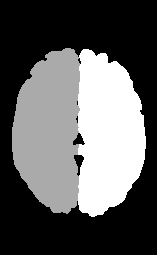
\includegraphics[width=.75in]{figures/label_bw}
                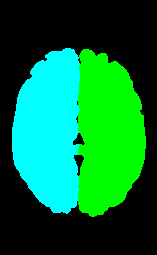
\includegraphics[width=.75in]{figures/label}
                \caption{Imagem segmentada antes e depois da coloração}
            \end{figure}

            Assim, antes de aplicar as cores da imagem segmentada ao modelo original, é necessário realizar a extração do corte do modelo original com a escala e normalização das intensidades de cada pixel, de modo que ambas as imagens (segmentada e original) estejam no mesmo intervalo. 

            Logo, a seguinte função com seu respectivo algoritmo é utilizada para aplicar as cores da imagem segmentada ao modelo original: \\

            \texttt{void apply\_mask(GrayImage* img, ColorImage* c\_img)}
            \begin{enumerate}
                \item Todos os valores de $R$, $G$, $B$ (imagem segmentada) e $I(p)$ (imagem original) são normalizados de $0$ a $1$;
                \item Os valores $RGB$ são convertidos para $YCgCo$;
                \item O $Y$ é substituído por $I(p)$ e os valores de $Cg$ e $Co$ são multiplicados por $I(p)$;
                \item Os novos valores de $YCgCo$ são convertidos novamente para $RGB$, ainda normalizados;
                \item Multiplica-se os valores de $RGB$ por $H$ e obtemos a nova imagem. \\
            \end{enumerate} 

            O resultado final é apresentado abaixo:

            \begin{figure}[ht!]
                \centering
                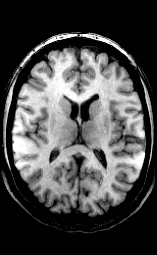
\includegraphics[width=.75in]{figures/example}
                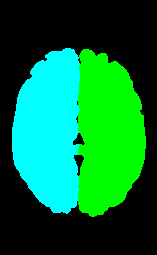
\includegraphics[width=.75in]{figures/label}
                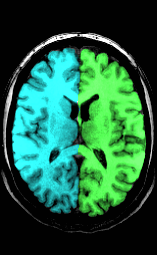
\includegraphics[width=.75in]{figures/color}
                \caption{Aplicação da máscara colorida no modelo original}
            \end{figure}


    \subsection{Demonstração: corte, coloração, brilho e contraste}
        Foi realizada uma aplicação em \textit{python} que garantisse a interação mais fácil do usuário com os métodos de visualização da imagem volumétrica. 

        A partir dos códigos em $C$ que realiza as manipulações gráficas, foi utilizada a interface em \textit{python} \textbf{Tkinter} para oferecer botões e uma interação mais responsiva ao uso da API, bastando a comunicação com os programas já compilados em $C$.

        \begin{figure}[ht!]
            \centering
            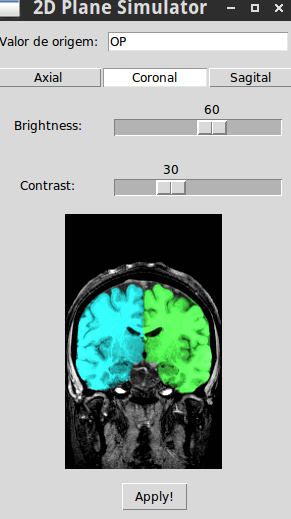
\includegraphics[width=1.1in]{figures/UI_BC}
            \caption{Exemplo da interface utilizada com o modelo \textbf{brain.scn}}
        \end{figure}

    \subsection{Wireframe}
        \subsubsection{Algoritmo}
            A implementação do wireframe foi feita a partir de um modelo e um vetor de visualização, ao qual é utilizado para extrair os ângulos $\theta_x$ e $\theta_y$. O algoritmo se baseou em:

            \begin{itemize}
                \item Dada a transformação \textbf{$\Phi$} em \textbf{$P = (x, y, z)$}: \\
                \begin{equation}
                \Phi(P) = T(q_c)R_y(\theta_y)R_x(\theta_x)T(-p_c)P^{T}
                \end{equation}
                \item Aplica a transformação \textbf{$\Phi$} em cada um dos vetores das seis faces do modelo e descobre quais faces são visíveis;
                \item Aplica a transformação \textbf{$\Phi$} nos vértices das faces visíveis;
                \item Realiza o algoritmo de \textbf{DDA} para todas as arestas visíveis, de $\Phi(P_1)$ a $\Phi(P_n)$.
            \end{itemize}

        \subsubsection{Demonstração}
            O resultado foi ilustrado a partir da mesma library em \textit{python} utilizada anteriormente, \textbf{Tkinter}. O usuário pode ajustar o vetor de visualização e produzir o wireframe correspondente, com uma cor gerada aleatoriamente.

            \begin{figure}[ht!]
                \centering
                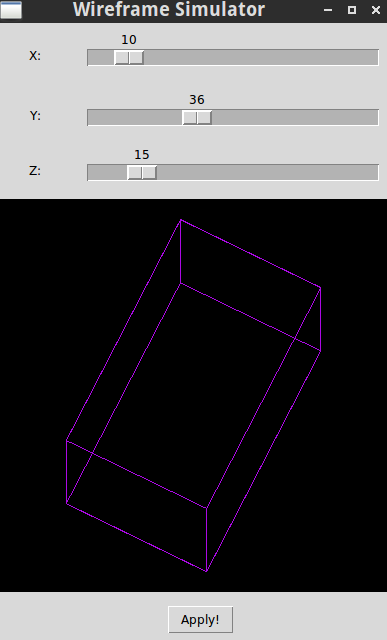
\includegraphics[width=1.1in]{figures/wire_interface}
                \caption{Exemplo da interface utilizada com o modelo \textbf{brain.scn}}
            \end{figure}

    \subsection{Corte planar}
        \subsubsection{Algoritmo}
            O corte planar é uma versão mais específica do corte em imagem 2D, apresentado anteriormente: ele permite a escolha de um ponto de referência $p_1$ e um vetor de visualização, garantindo maior liberdade de customização ao usuário. O algoritmo consiste em:

            \begin{itemize}
                \item Utiliza a transformação \textbf{$\Phi^{-1}(P)$} em dado ponto \textbf{$P = (x, y, z)$} e 
                $q_c = (\frac{D}{2}, \frac{D}{2}, -\frac{D}{2})$, com $D$ sendo a diagonal do modelo: \\
                    \begin{equation}
                        \Phi^{-1}(P) = T(p_1)R^{-1}T(-q_c)P^{T}
                    \end{equation}
                \item Determina $\alpha_x$, $\alpha_y$ e $\alpha_z$ para realizar as rotações adequadas;
                \item Aplica a transformação em todos os pontos $P$ da imagem de tamanho $I = (D, D)$, de forma a capturar o pixel correspondente da cena;
                \item Utiliza algoritmo de interpolação para capturar intensidade adequada do pixel, a partir da cena.
            \end{itemize}

        \subsubsection{Demonstração}
            Os testes para verificar corretude foram obtidos a partir do modelo de cubo, e posteriormente aplicados a modelos mais robustos a partir da interface interativa.

            \begin{figure}[ht!]
                \centering
                
\includegraphics[width=2in]{figures/planar}
                \caption{Cortes realizados na imagem cúbica}
            \end{figure}

            \begin{figure}[ht!]
                \centering
                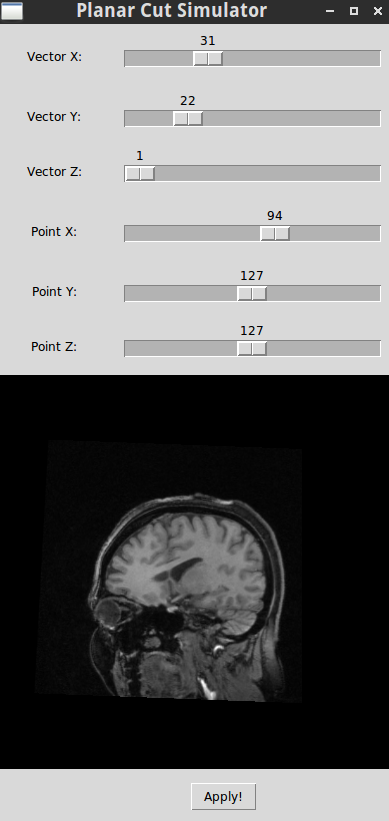
\includegraphics[width=1.1in]{figures/planar_interface}
                \caption{Exemplo de interface com o modelo \textbf{brain.scn}}
            \end{figure}

    \subsection{Reformatação planar}
        \subsubsection{Algoritmo}
            A reformatação planar proposta como projeto se baseia na obtenção de $n$ cortes planares e \textbf{ortogonais} entre o segmento de $p_1$ e $p_n$. Dessa forma, a entrada fornecida pelo usuário se baseia na cena original, o número $n$ de cortes, além dos pontos $p_1$ e $p_n$. O algoritmo se comporta em:

            \begin{itemize}
                \item Inicialmente, é obtido o vetor $\overrightarrow{v} = \cfrac{p_n - p_1}{||p_n - p_1||}$, utilizado como referência para realizar o corte planar.
                \item É estimado os valores ($dx$, $dy$, $dz$), com $dz < ||p_n - p_1||$. É aplicado um algoritmo parecido com o \textbf{DDA}, o qual decompõe $\lambda$ em $n$ valores, tais que $p_n = p_1 + n\cdot\lambda\overrightarrow{v}$.
                \item Em seguida, são extraídos os $n$ cortes da cena para cada valor de $i\cdot\lambda$, com $i \in \{1...n\}$. O corte planar resultante é acrescentado à imagem final, por meio de uma operação que verifica o valor de cada pixel entre o novo corte planar e a imagem resultante. 
                \begin{itemize}
                    \item Para cada valor do pixel $p \in (D, I)$ em ambas as imagens (as quais possuem a mesma dimensão): caso o valor do pixel no novo corte seja maior que um determinado \textbf{threshold} (como, por exemplo, o valor $200$), o valor é acrescentado à imagem final.
                \end{itemize}
            \end{itemize}

        \subsubsection{Demonstração}
            Como saída final, foram obtidos dois resultados distintos, uma vez que não estava muito claro qual seria o resultado esperado. O primeiro possui cortes de $p_1$ a $p_n$ sucessivos, os quais possuem as dimensões interpoladas durante a extração dos cortes. O segundo possui cortes de $p_1$ a $p_n$ em $n$ intervalos, não necessariamente sucessivos.

            \begin{figure}[!ht]
                \centering
                \subfloat[Cortes sucessivos]{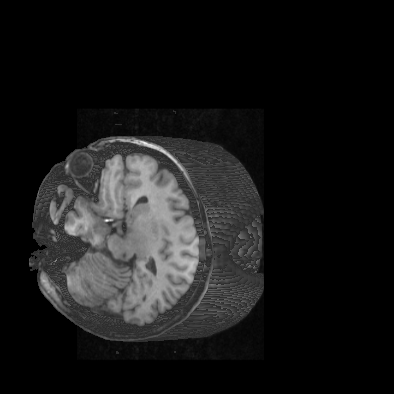
\includegraphics[width=1.1in]{figures/reformat_s}\label{fig:f1}}
                \hfill
                \subfloat[$n$ cortes]{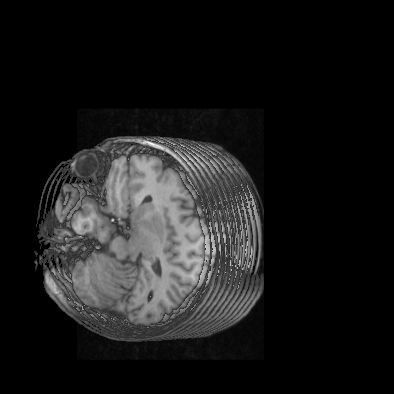
\includegraphics[width=1.1in]{figures/reformat_n}\label{fig:f2}}
                \caption{Resultados obtidos após a aplicação do algoritmo de reformatação planar}
            \end{figure}

    \subsection{Average e Maximum Intensity Projection}
        \subsubsection{Algoritmo}
            A realização de \textit{Average} e \textit{Maximum Intensity Projection} é feita a partir de um vetor de visualização, que representa o ponto de vista do usuário em relação ao modelo (utilizado para obter os ângulos $\theta_x$ e $\theta_y$). O algoritmo consiste em:

            \begin{itemize}
                \item Utiliza a transformação \textbf{$\Phi^{-1}(P)$} em dado ponto \textbf{$P = (x, y, z)$}, 
                $q_c = (\frac{D}{2}, \frac{D}{2}, \frac{D}{2})$ e $p_c = (-\frac{x}{2}, -\frac{y}{2}, -\frac{z}{2})$, com $D$ sendo a diagonal do modelo, $x$, $y$ e $z$ as dimensões que representam o tamanho do modelo: \\
                \begin{equation}
                    \Phi^{-1}(P) = T(-p_c)R_x^{-1}(\theta_x)R_y^{-1}(\theta_y)T(-q_c)P^{T}
                \end{equation}
                \item Aplica a transformação em cada ponto $P$ da imagem de tamanho $I = (D, D)$ e em $n = (0, 0, 1)$, de forma a obter o plano de visualização do usuário;
                \item Ainda em cada ponto $P$, aplica-se a seguinte relação de forma a descobrir o valores de $\lambda$ para os pontos $p_1$ e $p_n$, para cada face $j \in \{1 ... 6\}$:
                \begin{equation}
                    \lambda = \cfrac{\overrightarrow{n_j} \cdot (c_j - \Phi^{-1}(P))}{\overrightarrow{n_j} \cdot \Phi^{-1}(n)}
                \end{equation}
                A partir de $\lambda$, é adquirido o ponto $Q = \Phi^{-1}(P) + \lambda \cdot \Phi^{-1}(n)$, se $Q$ estiver dentro do domínio da cena, $\lambda$ é adotado como um candidato válido para $p_1$ e $p_n$.
                O menor e maior $\lambda$ encontrados correspondem a $p_1$ e $p_n$, respectivamente.
                \item Enfim, é aplicado o algoritmo de \textbf{DDA} para cada ponto $P$: para adquirir o \textit{Maximum Intensity Projection}, basta retornar o maior valor encontrado, enquanto para adquirir o \textit{Average Intensity Projection}, é retornado o valor médio entre todas as intensidades encontradas.
            \end{itemize}

        \subsubsection{Demonstração}
            A verificação de corretude foi feita com o modelo \textbf{brain.scn}, a partir da mesma interface em \textit{python} aplicada nos projetos anteriores.

            \begin{figure}[ht!]
                \centering
                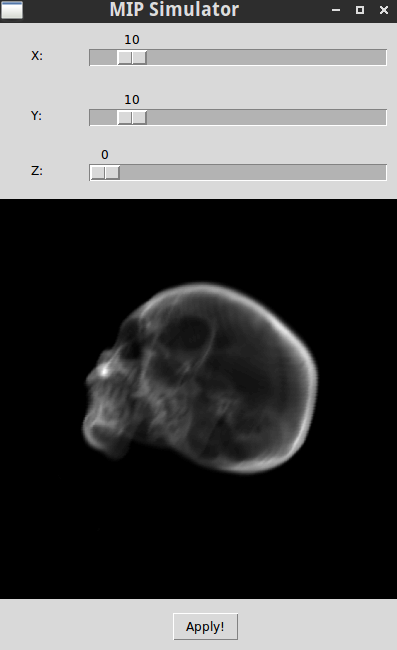
\includegraphics[width=1.1in]{figures/mip_avg}
                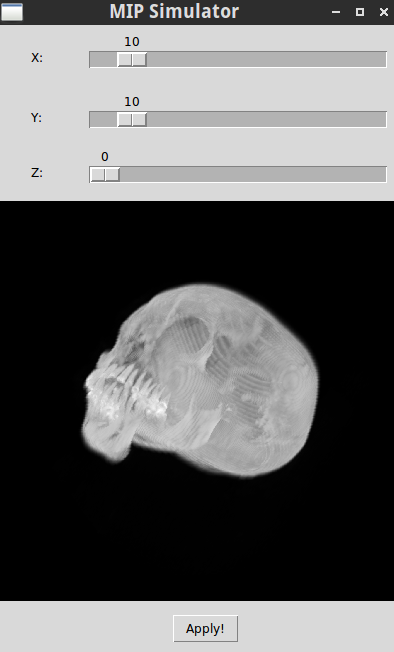
\includegraphics[width=1.1in]{figures/mip_max}
                \caption{Exemplo de interface com o modelo \textbf{brain.scn} com \textit{Average} e \textit{Maximum Intensity Projection}, respectivamente}
            \end{figure}

    \subsection{Rendering}
        \subsubsection{Algoritmo}
            O processo de realização do \textit{rendering} se originou de um algoritmo bastante semelhante ao apresentado anteriormente, utilizado para extrair o \textit{Average} e \textit{Maximum Intensity Projection}. As únicas diferenças estão no input (uma máscara de \textit{labels} é fornecida como entrada, além da cena original) e no último passo, ao aplicar o algoritmo \textbf{DDA}, que se comporta da seguinte maneira:

            \begin{itemize}
                \item Após obter os pontos $p_1$ e $p_n$, o algoritmo \textbf{DDA} é aplicado. Para cada ponto $p$ percorrido na função \textbf{DDA}, é verificado se os seus vizinhos esféricos de raio 1 possuem uma \textit{label} de objeto. Caso positivo, esse ponto vizinho é tomado como novo ponto de referência $p$ e é retornado $L(p)$ como valor final.
                \item O modelo de Phong aplicado em $p$, $L(p)$, corresponde a:

                \begin{equation}
                    L(p) = k_aL_a + D(p)(k_d\cos(\theta) + k_s\cos^{n_s}(2\theta))
                \end{equation}

                No modelo, foi considerado $k_a = 0.2$, $k_d = 0.5$, $k_s = 0.3$ e $n_s = 5$. $L_a$ corresponde ao valor máximo de intensidade, isto é, $H$. Além disso, de forma a adquirir o valor correto de $L(p)$:
                \begin{itemize}
                    \item O valor de $N$, que seria a normal do ponto $p$ na cena, foi calculado a partir dos vizinhos esféricos de $p$, utilizando raio 6. Dessa forma, para cada um dos pontos vizinhos $v$, é somado à normal a derivada entre $p$ e $v$. Isto é:
                    \begin{equation}
                        N = \sum_{p_i = 1}^{v} \cfrac{f(p_i) \cdot \Delta_i}{2 \cdot ||\Delta_i||}
                    \end{equation}

                    Em que $\Delta_i = p_i - p$.

                    \item O valor de $\theta$, isto é, o ângulo entre o ponto de vista do usuário e a normal, foi obtido a partir de:
                    \begin{equation}
                        \theta = \cos^{-1}(-N \cdot \Phi^{-1}(n))
                    \end{equation}

                    Em que $N$ é a normal no ponto $p$ e $\Phi^{-1}(n)$ se trata do vetor de visualização, já rotacionado. Além disso, $L(p)$ só é calculado se $0 \leq \theta \leq \frac{\theta}{2}$, enquanto a componente especular ($k_s$) é calculada se $0 \leq \theta \leq \frac{\theta}{4}$.

                    \item Finalmente, o valor de $D(p)$ é obtido como:
                    \begin{equation}
                        D(p) = H (1 - 0.8 \cfrac{||p - \Phi^{-1}(q)||}{D} + 0.2)
                    \end{equation}

                    Em que $\Phi^{-1}(q)$ é o ponto do plano de visualização (rotacionado e transladado), enquanto $D$ se trata da diagonal da cena.

                \end{itemize}
            \end{itemize}

        \subsubsection{Demonstração}
            A seguir estão os resultados de cada uma das componentes utilizadas para o cálculo de $L(p)$, garantindo o resultado do \textit{rendering}. 
            
            Além disso, também foi aplicada uma interface para a realização de testes e facilitar a manipulação dos resultados, também demonstrada a seguir.

            \begin{figure}[!ht]
                \centering
                \subfloat[$L(p)$]{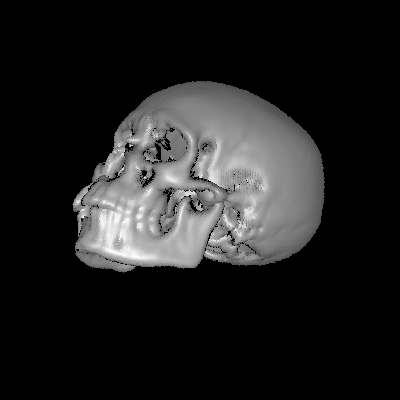
\includegraphics[width=1.1in]{figures/r_final}\label{fig:f1}}
                \hfill
                \subfloat[$k_aL_a$]{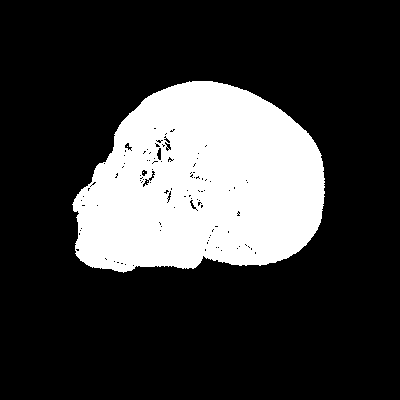
\includegraphics[width=1.1in]{figures/r_kala}\label{fig:f2}}
                \hfill
                \subfloat[$D(p)$]{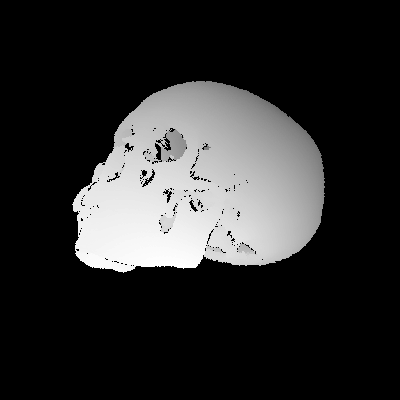
\includegraphics[width=1.1in]{figures/r_dist}\label{fig:f3}}
                \hfill
                \subfloat[$D(p)k_d\cos(\theta)$]{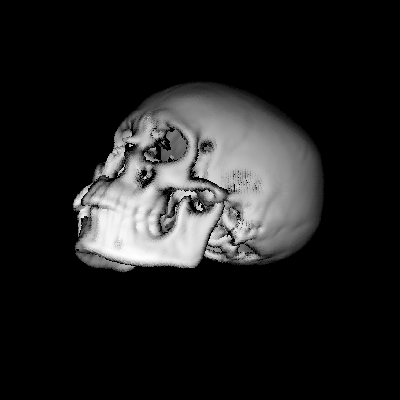
\includegraphics[width=1.1in]{figures/r_kd}\label{fig:f4}}
                \hfill
                \subfloat[$D(p)k_s\cos^{n_s}(2\theta)$]{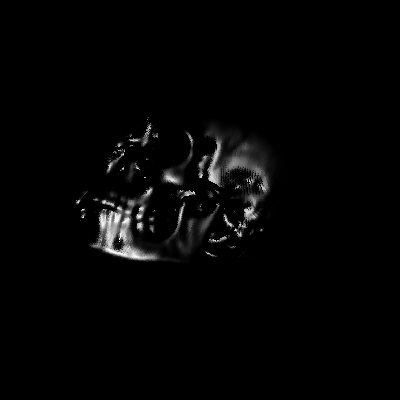
\includegraphics[width=1.1in]{figures/r_ks}\label{fig:f5}}
                \caption{Demonstração de cada estágio do processo de renderização}
            \end{figure}

            \begin{figure}[ht!]
                \centering
                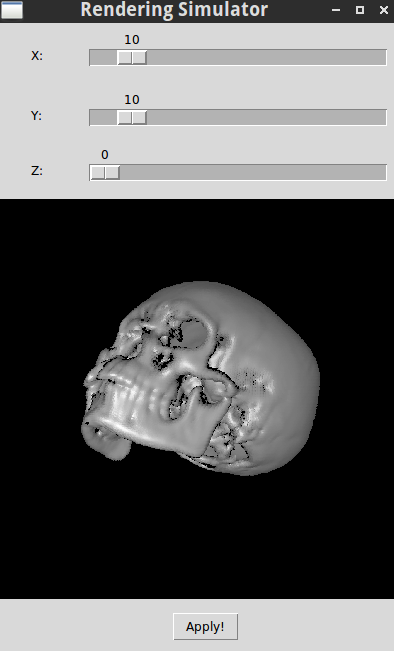
\includegraphics[width=1.1in]{figures/r_interface}
                \caption{Interface com o modelo \textbf{skull.scn} para o \textit{rendering}}
            \end{figure}

            É possível observar que o resultado final possui alguns pixels irregulares (com a mesma cor do fundo) entre as bordas do modelo. A ocorrência desses pixels se deve, principalmente, à precisão da normal, derivada da aproximação do ponto $p$. De modo a corrigir este problema, deveria ter sido aplicado uma função de interpolação entre todas as normais vizinhas ao ponto $p$, ainda no \textbf{DDA}, além da identificação da máscara adequada, também utilizando a interpolação. Como o processamento iria tomar muito tempo com esse procedimento, o qual exigiria técnicas de paralelização para uma execução viável, o resultado final foi o aproximado.

    \subsection{Rendering com opacidade}
        \subsubsection{Algoritmo}
            Novamente, o algoritmo para a aplicação do \textit{rendering} com opacidade se deriva do próprio algoritmo do \textit{rendering}, demonstrado anteriormente. As entradas são as mesmas (vetor de visualização, cena original e cena com máscaras de objeto) - entretanto, a diferença está na forma em que o \textbf{DDA} retorna o valor de intensidade:

            \begin{itemize}
                \item Para cada ponto $p$ percorrido na função \textbf{DDA}, é verificado se os seus vizinhos esféricos de raio 1 possuem valor diferente da \textit{label} atual e da \textit{label} do fundo da cena, e que não tenha sido percorrido anteriormente.

                \begin{itemize}
                    \item Caso positivo, esse ponto vizinho é tomado como novo ponto de referência $p_i$.
                    \begin{itemize}
                        \item Caso seja a primeira ocorrência de um novo objeto ($i = 1$), é adicionado $\alpha_1 L(p_1)$ ao valor final. 

                        \item Caso contrário, é adicionado $\alpha_i L(p_i) + \prod_{j = 1}^{i - 1}(1 - \alpha_j)$ ao valor final. Cada valor $\alpha_j \in [0, 1]$ corresponde ao valor de opacidade do objeto $j$.
                    \end{itemize}

                    \item Caso contrário, apenas ignore e continue a função.
                \end{itemize}

                \item O valor final é retornado após atingir o ponto $p_n$.
            \end{itemize}

        \subsubsection{Demonstração}
            Os resultados e problemas encontrados são semelhantes aos do \textit{rendering}. A seguir, é apresentada a interface com o modelo \textbf{brain.scn}, o qual possui diferentes objetos na cena e permite uma melhor visualização de opacidade.

            \begin{figure}[ht!]
                \centering
                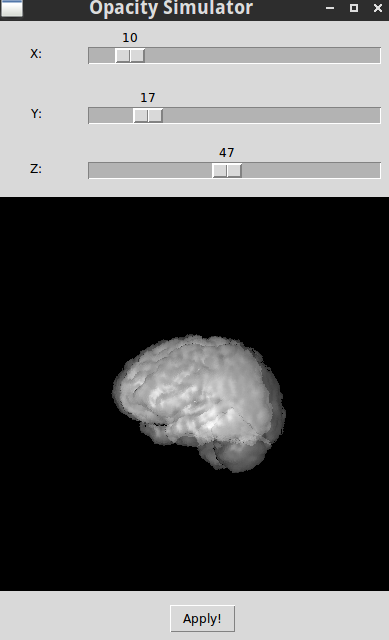
\includegraphics[width=1.1in]{figures/o_interface}
                \caption{Interface com o modelo \textbf{brain.scn} para o \textit{rendering} com opacidade (em que cada $\alpha_j$ possui valor $0.4$)}
            \end{figure}

\section{Conclusão} \label{sec:int}
    Foram apresentados os diversos projetos apresentados na disciplina que dizem respeito à manipulação de imagens volumétricas. Finalmente, é importante ressaltar que todo código e material utilizado se encontra no repositório da disciplina \cite{REPO}.

\bibliography{bib/tasklab} 
\bibliographystyle{ieeetr}

\end{document}
